\section{Preferential attachment: \emph{"The rich get richer"}}
\label{sec:burstiness}

The term \textit{burstiness} describes the fact that some events appear in bursts, \textit{i.e.} once they appear, they are more likely to appear again. The notion of burstiness is similar to the one of aftereffect of future sampling \cite{feller_68}, which describes the fact that the more we observe an event, the higher the expectation to find new occurrences of this event. In (social) network studies, the burstiness effect is alos referred to as \textit{preferential attachment}\footnote{A.L. Barab\'asi, for example, uses the term \textit{preferential attachement} in \cite{barabasi1999emergence}, and \textit{burstiness} in \cite{barabasi_burst}.}: a node with many connections is more likely to have new connections than a node with few connections. To take into account this behavior, in the network generative model  (BA) \cite{albert2002statistical} model, a node is connected to an existing target node with a probability proportional to the number of links of the target node. This leads to scale-free networks that are characterized by a heavy tailed degree distribution, which can be approximated by a power law distribution such that the fraction of nodes $\pr(d)$ having a degree $d$ follows a power law $d^{-\gamma}$, where $\gamma$ typically ranges between 2 and 3~\cite{barabasi1999emergence}. 

Burstiness has been studied in different fields, in particular in computational linguistics and information retrieval to characterize word occurrences \cite{church1995poisson}. In these domains, simple definitions of burstiness, that directly capture the fact that a probability distribution is bursty if the probability of generating a new occurrences of an event increases with the number of occurrences of this event, have been proposed\cite{clinchant2008bnb,clinchant2010information}. We rely here on the discrete version of theses definitions, which takes the following form:
%
\begin{definition}[Burstiness]
	A discrete distribution $\pr$ is bursty if and only if, for all integers $(n, n')$, $n \geq n'$ :
	\begin{equation}
	\pr(X \geq n+1 \mid X \geq n) > \pr(X \geq n'+1 \mid X \geq n') \nonumber
	\end{equation}
	where $X$ denotes a random variable.
\label{def:burst}
\end{definition}
%
In the context of social networks, the notion of burstiness, or preferential attachement, appears at different levels: (a) a global preferential attachment level that characterizes the degree distribution of nodes in the network, (b) a local preferential attachment level that characterizes the degree distribution of nodes within communities, and (c) a class/feature burstiness level that characterizes the distributions of nodes among latent classes/features. We provide below a formal definition of these elements.
%


\begin{definition}[Burstiness in social networks]
Let $i$ be a node in a social network $G=(V,E)$, and let $d_i$ denote its degree. Furthermore, let $\mathcal{M}=\{\M_e, \M_g\}$ be a link prediction model as defined in Section~\ref{sec:models}.
\begin{description}
 \item[(i)] \emph{Global Preferential Attachment}: we say that $\mathcal{M}$ satisfies the global preferential attachement iff, for any node $j \in V$ not connected to $i$, $\pr(y_{ij}=1 \mid d_i \ge n, \M)$ increases with $n$.
 \item[(ii)] \emph{Local Preferential Attachment}: we say that $\mathcal{M}$ satisfies the local preferential attachement iff, for any node $j \in V$ not connected to $i$ and belonging to the same community as $i$, $\pr(y_{ij}=1 \mid d_{i,c} \ge n, \M$ increases with $n$; $d_{i,c}$ denotes the degree of node $i$ in its community.
  \item[(iii)] \emph{Class/Feature Burstiness}: we say that $\mathcal{M}$ satisfies the feature/class burstiness effect, iff, for any node $i$ and latent class/feature $k$, $\pr(f_{ik} > 0 \mid \mat{f}_{\bm{.}k}^{-ik} \ge n, \M)$ increases with $n$; where $\mat{f}_{\bm{.}k}^{-ik}$ denotes the number of nodes, other than node $i$, assigned to latent class/feature $k$ in the network.
\end{description}
\label{def:burst-soc-net}
\end{definition}
%
There are two things to note here. The first one is that $f_{ik}$ in (iii) equals $1$ for ILFM (as it relies on binary features), and is in $[0,1]$ for IMMSB. The second one is that the fact that the probability $\pr(y_{ij}=1 \mid d_i \ge n, \M)$ increases with $n$ is equivalent to the fact that the probability $\pr(d_{i} \ge n+1 \mid d_i \ge n, \M)$ increases with $n$. Indeed:






\begin{theorem}
	 Given a the distribution $p(d_i=n)$  of a degree $d_i \quad \forall i \in E$, for any joint exchangeable graph $G(V,E)$, then if $n >> 0$ the distribution $p$ is c-bursty iff (\textcolor{red}{Need to introduce this definition of the burstiness, who said that a distribution is c-bursty if it a exist a integer $c$ such that the distribution is bursty for all $n > c$}) :
	\begin{align}
	  \Delta_n \p(y_{ij}=1 | d_i^{n}) > 0
	\end{align}
	Where $d_i^{N,n}$ represent the set node $j' \in E \\ j$n with $n$ element taking value 1 and $d_i=n$.
\end{theorem}

\begin{proof}
	First we recall that for a jointly exchangeable graph, we have that:
	\begin{equation*}
	\p(y_{ij}: (i,j) \in V^2) = \p(y_{\sigma(i)\sigma(j)}: (i,j) \in V^2)
	\end{equation*}
	For any permutation $\sigma$ of the integer $\{1,..,n\}$. Furthermore it can be show that $ \pr(d_i \geq n'+1 \mid d_i \geq n')$ and $\frac{\p(d_i=n+1)}{\p(d_i=n)}$ vary in the same direction with $n$ (Clinchant 2006). Under the exchangeability assumptions, one can write that:
	
	\begin{align*}
	 b_n=\frac{\p(d_i=n+1)}{\p(d_i=n)} = \frac{\dbinom{N+1}{n+1} p(d_i^{N+1,n+1})}{\dbinom{N}{n} p(d_i^{N,n})}
	\end{align*}
	This equation reflect the fact that $\p(d_i=n+1)$ state for a new observation in the underlying random structure $d_i^{N,n}$. Applying a product rule, we have that:
	
	\begin{equation*}
	b_n = \frac{N+1}{n+1} \p(y_{ij}=1 | d_i^{N,n})
	\end{equation*}
	
	The differential is then equal to:
	\begin{align*}
	&\Delta_n b_n= b_{n+1} - b_n  \\
	&= \frac{N+1}{n+2} \p(y_{ij}=1 | d_i^{N,n+1}) - \frac{N+1}{n+1} \p(y_{ij}=1 | d_i^{N,n})
	\end{align*}
	
	The burstiness properties is statisfied iff $\forall n \in \mathbb{N}$:
	\begin{align*}
	\Delta_nb_n > 0 \iff \frac{n+1}{n+2}\p(y_{ij}=1 | d_i^{N,n+1})  > \p(y_{ij}=1 | d_i^{N,n})
	\end{align*}
	
	The last equation show that the burstiness condition holds if $n >> 0$.
	\textcolor{red}{Est ce qu'avec le passage au limite je ne perds pas l'inégalité strict de la definition ? (surement) donc ca renvoit à la note du haut concernant un borne...}

\label{b-theorem}
\end{proof}

The above definitions, characterizing probabilistic link models according to burstiness in social networks, are thus directly related to the general definition of burstiness given in Definition~\ref{def:burst}. Note that the theorem \ref{b-theorem} reflect the fact there is is a cut-off where a distribution loose if bursty aspect. This is illustrated by the power law distribution that need such cut-off because a distribution nned to sum to one  \ref{clauset2009power}.


\begin{proposition}
	The IMMSB models satisfy the local preferential attachments in the generative mode $\M_g$.
\end{proposition}

\begin{proof}
We have:
In IMMSB one can write the predictive distribution conditionned by $d_i^{N,n}$:

\begin{equation} 
p(y_{ij} = 1 | d_i^{N,n}, \mathcal{M}) = \int_{\Theta} p(y_{ij}=1|\Theta) \frac{p(d_i^{N,n} | \Theta)}{pd_i^{N,n}} p(\Theta) d\Theta \nonumber
\end{equation}

By only restraining the relations that occur inside class $c=\{k,k\}$, one can write the local preferential attachment:

\begin{align*} \label{eq:sum}
&p(y_{ij} = 1 | d_{ic}>n, \mathcal{M})  \\
&=  \frac{ \int_{\phi_{c}} p(y_{ij}=1|\phi_{c}) p(d_{ic}^{N,n} | \phi_{c}) p(\phi_{c}) d\phi_{c}}{\int_{\phi_{c}} \p(d_{ic}^{N,n} | \phi_{c}))       p(\phi_{c}) d\phi_{c}}   \\
&= \frac{ \text{beta}(n+1+\lambda_1, N-d_{ic}+\lambda_0) }{\text{beta}(n+\lambda_1, N-d_{ic}+\lambda_0) } 
\end{align*}


\end{proof}

\begin{proposition}
	The ILFM models statisfy the local preferential attachments. in the generative mode $\M_g$.
\end{proposition}
\begin{proof}
	\textcolor{red}{This is not sure actually, local proof for ILFM to finish...}
\end{proof}

\begin{proposition}
	The ILFM and IMMDB models do not statisfy the global and local preferential attachments. in the mode $\M_e$.
\end{proposition}

The proof of this statement is trivially true in the sens that given $\mat{F}$ and $\mat{\Theta}$, the link likelihood is fully determined and hence do not depend on new links being generated. 

\begin{proposition}
	Both ILFM and IMMSB models satisfy the feature burstiness.
\end{proposition}

The proof for this statement comes directly from the Diaconis-Ilvisaker results \cite{diaconis1979conjugate}. They state \emph{'subject to regularity conditions, the conjugate priors typically used satisfy, and are characterized by, a  similar relation of posterior linearity'}:
\begin{equation}
\E[\E[X\mid \Theta] \mid X=x] = ax+b \quad \text{for} \quad x=0,1,2,... \nonumber
\end{equation}

Especially, the Dirichlet Process and the Indian Buffet Process, as prior for the latent features, are typically build on the suitable conjugate distribution respectively Dirichlet-Multinomial and Beta-Bernoulli. Furthermore, this claim is highlighted by the Gibbs update that corroborate the feature burstiness effect:
\begin{align}
&\p(f_{ik} = 1 | F^{-ik}) = \frac{m_k^{-ik}}{N} \qquad \text{ILFM feature update} \nonumber \\
&\p(f_{ik} = 1 | F^{-ik}) = \frac{n_{ik}^{-z_{ij}}+\alpha_k}{N+\alpha_.} \qquad \text{IMMSB feature update} \nonumber \\
\end{align}

Where the $m_k^{-ik}$ described the number of elements that have the $k$-iem feature active except for element $i$, similarly $n_{ik}^{-z_{ij}}$ represents the number of times that $i$ was assigned to $k$ except for relation $(ij)$ (class membersehip are jointly sampled in MMSB).

In figure \ref{fig:gen_burst_mmsb} we represent tree networks generated by ILFM and iMMSB. We compute a goodness of fit to quantify the power law hypothesis on the empirical degree distributions. The protocol is described in section \ref{sec:experiments}. As an empirical illustration for our claims on preferential attachment, we show a 3*3 figure where each columns is particular setting of hyper-parameter and the rows are respectively, the global degree distribution, the local degree distribution and feature distribution (on a max a assignment point of view).

As we can see in the experiments, we can generate networks that do fit the burstiness definition on the overall degree distribution.

\begin{figure}[h]
	\centering
	
	\minipage{0.16\textwidth}
	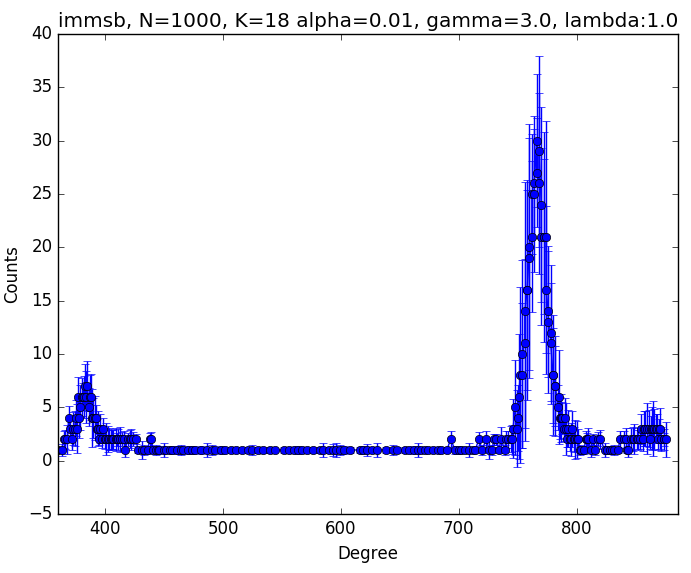
\includegraphics[width=3.2cm, height=3.7cm]{img/M_g_peaks/figure_1}
	\endminipage
		\minipage{0.16\textwidth}
	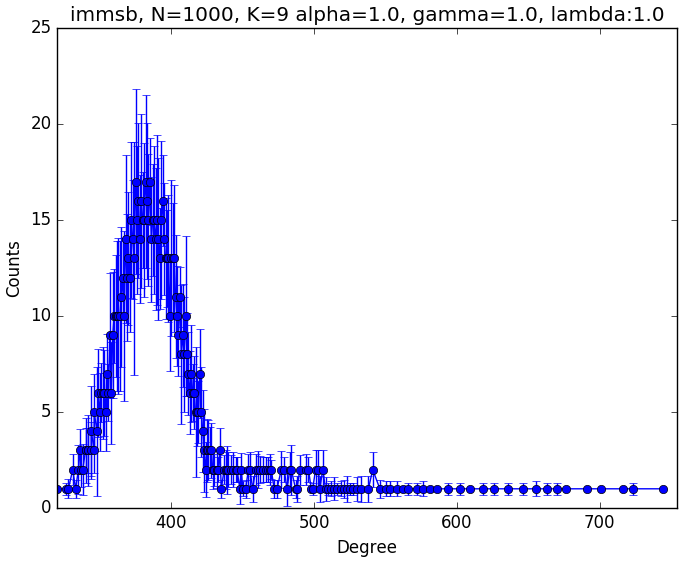
\includegraphics[width=3.2cm, height=3.7cm]{img/M_g_power_law/figure_1}
	\endminipage
	\minipage{0.16\textwidth}
	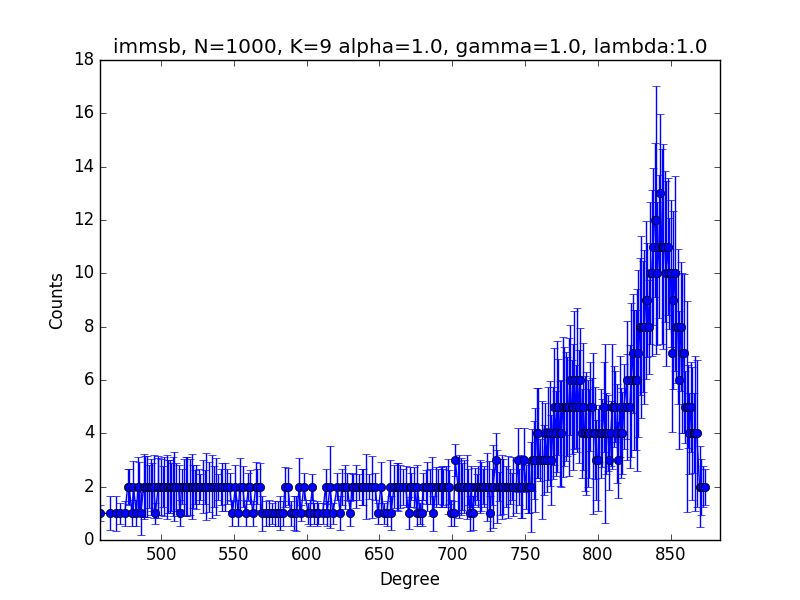
\includegraphics[width=3.2cm, height=3.7cm]{img/M_g_regular/figure_1}
	\endminipage
		\vspace{-0.4cm}
	\minipage{0.16\textwidth}
	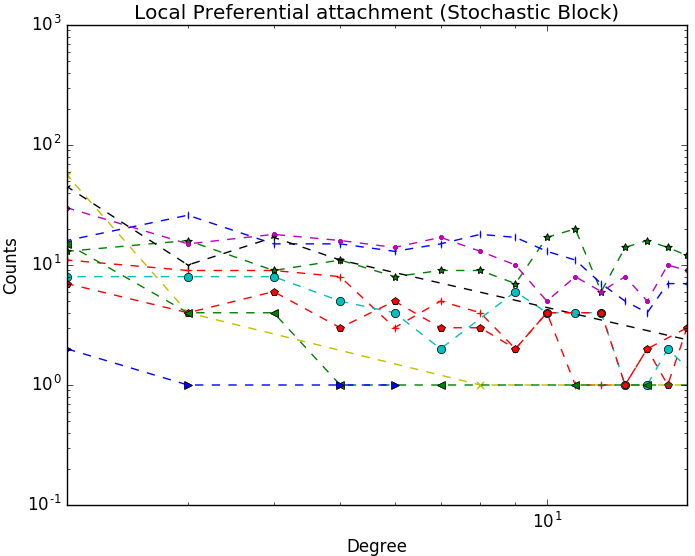
\includegraphics[width=3.2cm, height=3.7cm]{img/M_g_peaks/figure_3}
	\endminipage
		\minipage{0.16\textwidth}
	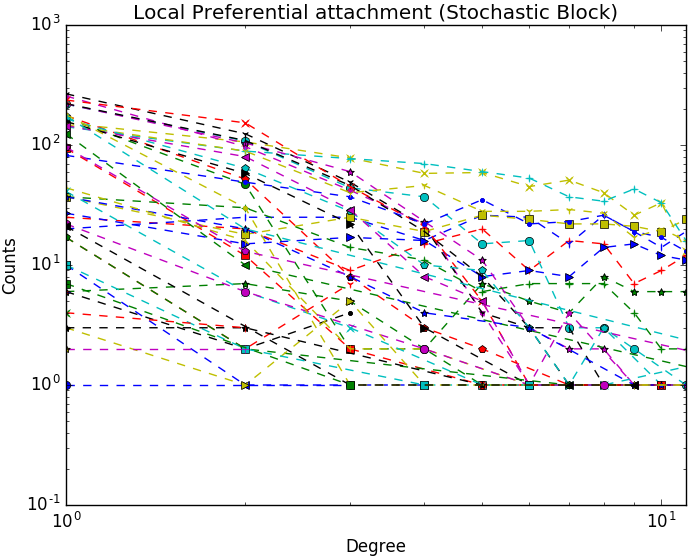
\includegraphics[width=3.2cm, height=3.7cm]{img/M_g_power_law/figure_3} 
	\endminipage
	\minipage{0.16\textwidth}
	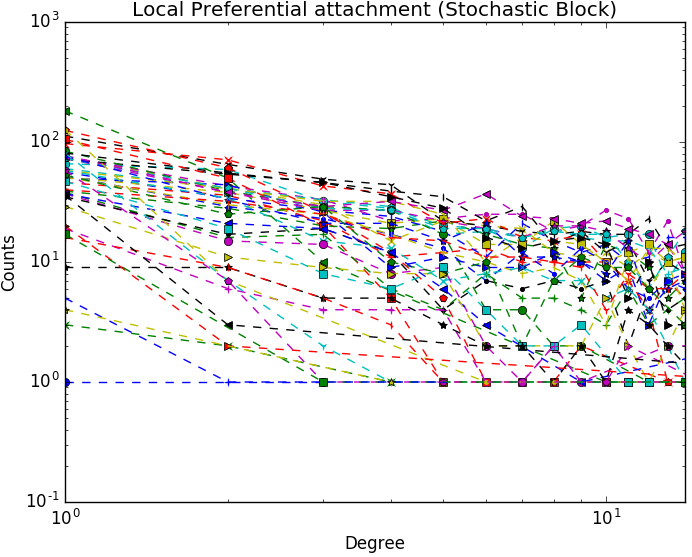
\includegraphics[width=3.2cm, height=3.7cm]{img/M_g_regular/figure_3}
	\endminipage
		\vspace{-0.4cm}
	\minipage{0.16\textwidth}
	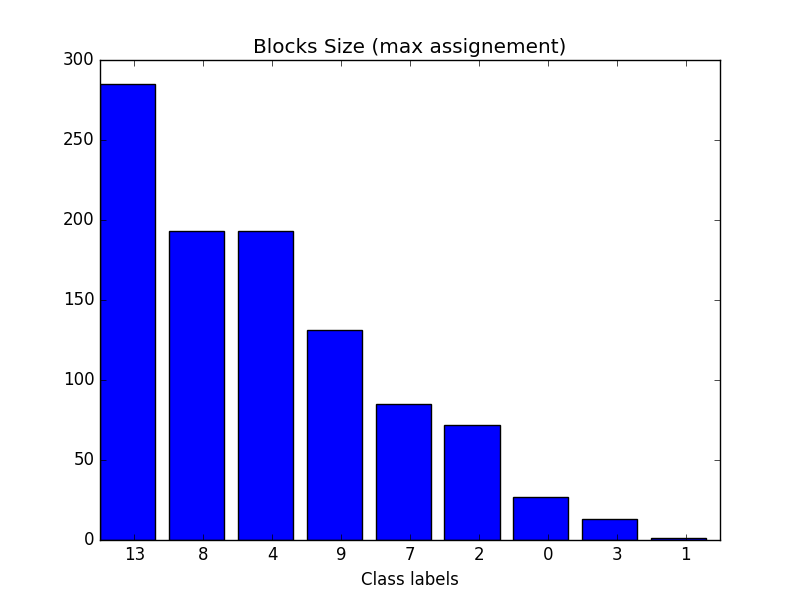
\includegraphics[width=3.2cm, height=3.7cm]{img/M_g_peaks/figure_5}
	\endminipage
	\minipage{0.16\textwidth}
	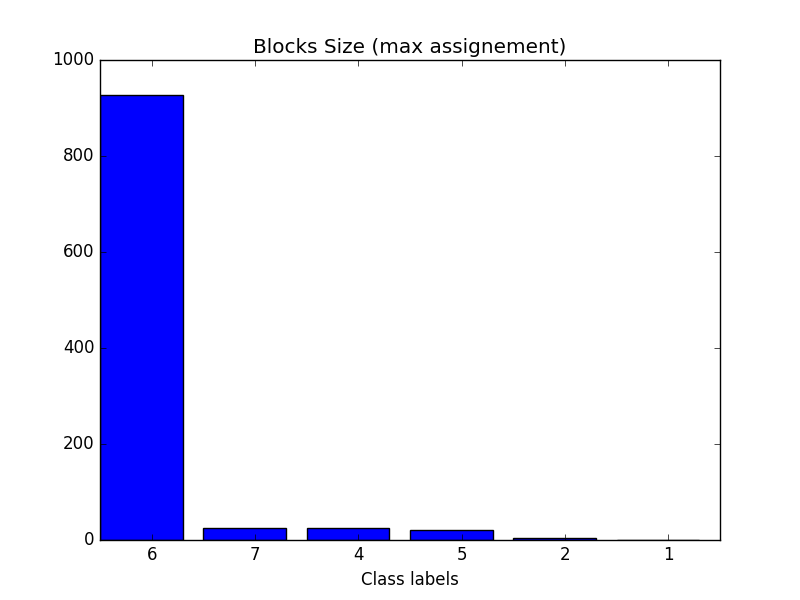
\includegraphics[width=3.2cm, height=3.7cm]{img/M_g_power_law/figure_5} 
	\endminipage
	\minipage{0.16\textwidth}
	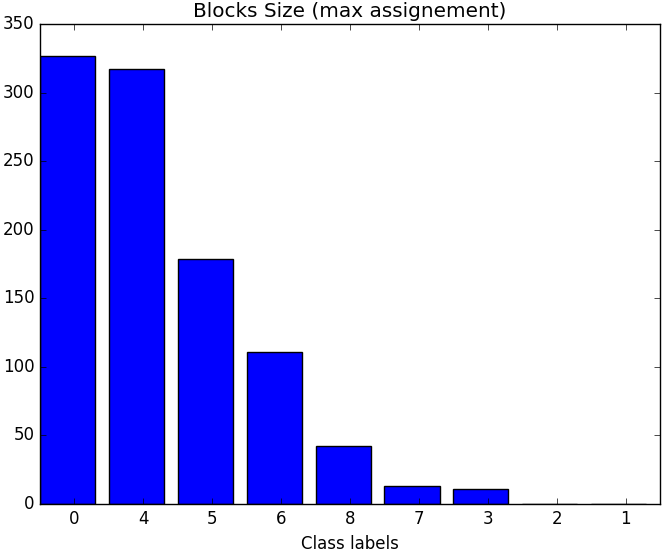
\includegraphics[width=3.2cm, height=3.7cm]{img/M_g_regular/figure_5}
	\endminipage
	\caption{Generated Networks with in three different settings (same set than for figure \ref{fig:gen_blocks}). The upper figures show the global preferentual attachment. The lower figures show the local preferential attachment. While global preferential attachment is not a pure features of model, we see that the local preferential attachment has linear form in the log-log space.}
	\label{fig:gen_burst_mmsb}
\end{figure}

%\paragraph{Remark}
%We see that is possible to generate networks that don't satisfy the global preferential effect...
\textcolor{red}{remark on the global preferential attachment, that is not satisify on the realisation of networks provided in figure 3 ?}


